%mark = star, diamond, square, otimes
%\documentclass{article}
%\usepackage{pgfplots}
%\usepackage[justification=centering]{caption}
%\pgfplotsset{compat=newest}
%\begin{document}
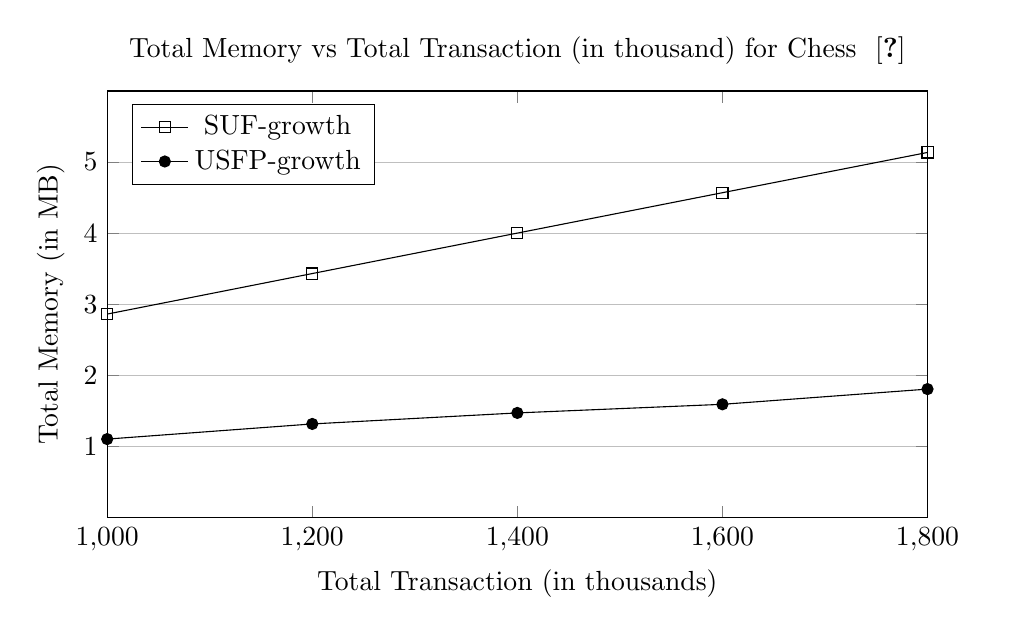
\begin{tikzpicture}
\begin{axis}[
	title={\parbox{\linewidth}{\centering Total Memory vs Total Transaction (in thousand) for Chess ~\cite{dataset}}},
	width=12cm,
	height=7cm,
    xlabel={Total Transaction (in thousands) },
    ylabel={Total Memory (in MB) },
    xmin=1000, xmax=1800,
    ymin=0, ymax=6,
    xtick={600,800,1000,1200,1400,1600,1800},
    ytick={1,2,3,4,5},
    legend pos=north west,
    ymajorgrids=true,
    grid style={line width=.2pt,draw=gray!50},
]
 
\addplot[
    solid, every mark/.append style={solid, fill=gray}, mark=square
    ]
    coordinates {
			(600,	1.720)
			(800,	2.291)
			(1000,	2.862)
			(1200,	3.432)
			(1400,	4.001)
			(1600,	4.569)
            (1800,	5.135)



	};
    \addlegendentry{SUF-growth}
\addplot[
    solid, every mark/.append style={solid, fill=black}, mark=*
    ]
    coordinates {
			(600,	0.681 )
			(800,	0.865 )
			(1000,	1.104 )
			(1200,	1.317 )
			(1400,	1.472 )
			(1600,	1.593 )
            (1800,	1.807 )


};
    \addlegendentry{USFP-growth}
 
\end{axis}
\end{tikzpicture}
%\end{document}